\documentclass[preprint,12pt]{elsarticle}

%% Essential packages
\usepackage{amssymb}
\usepackage{amsmath}
\usepackage{amsthm}
\usepackage{graphicx}
\usepackage{booktabs}
\usepackage{multirow}
\usepackage{array}
\usepackage{url}
\usepackage{xcolor}
\usepackage{subcaption}
\usepackage[hidelinks]{hyperref}

\journal{Biomedical Signal Processing and Control}

\begin{document}

\begin{frontmatter}

\title{ApproxDA-TransUNet: A highly efficient medical image segmentation method with dual spatial and channel attention approximation}

\author[inst1]{Author One\corref{cor1}}
\cortext[cor1]{Corresponding author}
\ead{author1@example.com}

\author[inst2]{Author Two}
\ead{author2@example.com}

\author[inst1]{Author Three}
\ead{author3@example.com}

\affiliation[inst1]{organization={Department of Computer Science, University Name},
            city={City},
            country={Country}}

\affiliation[inst2]{organization={Department of Biomedical Engineering, University Name},
            city={City},
            country={Country}}

\begin{abstract}
Dual-attention networks effectively capture spatial and channel-wise dependencies for medical image segmentation, but models like DA-TransUNet incur prohibitive computational overhead ($\approx$108M parameters, 30+ GFLOPs) due to full-map self-attention, heavy Vision Transformer encoders, and wide decoders. We present \textbf{ApproxDA-TransUNet}, an ultra-lightweight architecture engineered for clinical efficiency without sacrificing segmentation precision. ApproxDA-TransUNet integrates four synergistic designs: an early-truncated ResNet-50 stem (stride 8), a compact top-down LightViT-T bottleneck transformer, tri-axial dual-attention approximation blocks (local windowing $M=28$, low-rank subspace projection $r=32$, and grouped channels $G=8$), and a uniform $C=64$ slim decoder. Evaluated across five multi-modal benchmarks (Synapse CT, ACDC MRI, CVC-ClinicDB polyp, ISIC 2018 dermoscopy, and FeTA 2.4 fetal MRI) over three independent seeds, ApproxDA-TransUNet reduces parameters by $90.0\%$ ($10.75$M vs. $107.95$M) and compute by $77.1\%$ ($6.92$ vs. $30.25$ GFLOPs) while consistently outperforming DA-TransUNet (mean paired Dice gain $+0.37\%$, $p = 0.009$). On FeTA 2.4, it matches 3D volumetric baselines at $<2.5\%$ of their FLOPs. Mechanistic diagnostics reveal an $\alpha/\gamma$ gradient deadlock in SGD that renders raw attention matrices dormant, confirming that feature modulation is governed by internal bottleneck convolutions and explaining why aggressive approximation preserves full accuracy.
\end{abstract}

\begin{keyword}
Biomedical image segmentation \sep Lightweight architecture \sep Dual-attention approximation \sep Vision Transformer \sep Multi-organ segmentation
\end{keyword}

\end{frontmatter}

%% Sections
\section{Introduction}
\label{sec:introduction}

Automated biomedical image segmentation is fundamental to computer-assisted diagnosis, radiotherapy planning, and surgical navigation~\cite{ronneberger2015unet,zhou2018unetpp,chen2021transunet}. Clinical modalities span a broad spectrum---from 3D volumetric CT and MRI to 2D endoscopic video and high-resolution dermoscopy. Accurate boundary delineation across these domains requires architectures capable of both fine-grained edge localization and expansive global context modeling.

While convolutional neural networks (CNNs)~\cite{ronneberger2015unet,zhou2018unetpp,oktay2018attention} form the conventional baseline, their localized receptive fields limit long-range context aggregation. Hybrid CNN-Transformer frameworks like TransUNet~\cite{chen2021transunet} address this via self-attention, and dual-attention networks~\cite{fu2019dual} concurrently capture spatial affinities via Position Attention Modules (PAM) and cross-channel correlations via Channel Attention Modules (CAM). Recently, DA-TransUNet~\cite{sun2024datransunet} integrated dual-attention blocks across multi-scale skip connections and the bottleneck, demonstrating state-of-the-art accuracy on multi-organ CT and colon polyp benchmarks.

Despite their representational strength, standard dual-attention architectures are computationally heavy. Full-map PAM scales quadratically with the number of spatial tokens and CAM with the number of channels, and DA-TransUNet couples these modules with a ViT-B/16 encoder and a wide decoder, which brings it above 100M parameters and makes it costly to train and deploy on resource-constrained hardware. The quadratic cost of attention has prompted efficient approximations---windowed attention~\cite{liu2021swin}, low-rank factorization~\cite{wang2020linformer}, and grouped channel interaction~\cite{rahman2024emcad}---but in DA-TransUNet the dual-attention blocks account for less than $3\%$ of the parameters and FLOPs; most of the cost lies in the ViT-B/16 encoder and the wide decoder around them.

In our preliminary workshop study~\cite{zhong2026approxda}, we introduced the ApproxDA block, which keeps the DANet head of DA-TransUNet and replaces its attention operators with three independently controllable approximations: windowed position attention (window size $M$), low-rank projection (rank $r$), and grouped channel attention (groups $G$). In that study, exact attention showed no consistent advantage over its low-rank approximation, but the model kept the R50-ViT-B/16 backbone, so the savings of the approximated attention barely reached the whole network. In this work, we carry the approximated dual attention into a lightweight architecture. We present \textbf{ApproxDA-TransUNet}, a system-level redesign of DA-TransUNet built from four components:
(i) a \emph{ResNet-50 stem truncated after its second stage} followed by a compact Vision Transformer (\emph{LightViT-T}~\cite{huang2022lightvit}), which makes the encoder about ten times smaller;
(ii) \emph{approximated dual-attention blocks}, in which position attention is restricted to local windows and projected to a low rank, channel attention is computed in groups, and the two branches are blended with a fixed, equal gate;
(iii) these blocks on all three skip connections and on the bottleneck after the transformer, whereas DA-TransUNet applies dual attention to two of the skips and to the patch embeddings before the ViT; and
(iv) a \emph{slim decoder} with additive skip fusion and narrow channels at every skip stage.
Together, these changes reduce the parameters to ${\sim}10\%$, the FLOPs to ${\sim}23\%$, and the GPU memory for training and inference to ${\sim}42\%$ of those of DA-TransUNet.

In single-axis ablations on Synapse, removing the dual-attention blocks costs nearly three Dice points, whereas their approximation costs no accuracy: the exact global dual attention of DA-TransUNet gives the same Dice with more computation and twice the training time.

We evaluate ApproxDA-TransUNet with three seeds on five benchmarks spanning CT, cardiac MRI, colonoscopy, dermoscopy, and fetal brain MRI: Synapse, ACDC, CVC-ClinicDB, ISIC 2018, and FeTA 2.4. Its mean Dice is higher than that of DA-TransUNet on all five datasets, by $0.37$ points on average; the gain on any single dataset is within seed variation. On FeTA 2.4, it is about two points above the reproduced U-Net family and Swin-Unet and on par with TransUNet, at a tenth of TransUNet's size.

The primary contributions of this paper are:
\begin{itemize}
    \item \textbf{Lightweight dual-attention architecture}: ApproxDA-TransUNet retains the dual attention of DA-TransUNet with ${\sim}10\%$ of its parameters, ${\sim}23\%$ of its FLOPs, and ${\sim}42\%$ of its GPU memory, at comparable segmentation accuracy, making dual-attention segmentation practical on modest clinical hardware.
    \item \textbf{Dual-attention approximation}: windowed low-rank position attention ($M$, $r$) and grouped channel attention ($G$) as three independently parameterized axes, with single-axis ablations on Synapse showing that the blocks are needed and that the approximation matches exact dual attention at lower cost.
    \item \textbf{Five-dataset, three-seed validation}: paired comparisons with DA-TransUNet on benchmarks spanning CT, MRI, colonoscopy, dermoscopy, and fetal MRI, with literature and reproduced baselines and a deployment profile.
\end{itemize}

The rest of this paper is organized as follows: Section~\ref{sec:related_work} reviews related work; Section~\ref{sec:method} presents the methodology; Section~\ref{sec:experiments} reports experimental results; Section~\ref{sec:ablation} provides ablation studies; Section~\ref{sec:discussion} discusses augmentation, deployment cost, and limitations; Section~\ref{sec:conclusion} concludes the paper.

\section{Related Work}
\label{sec:related_work}

\subsection{Architectures for Biomedical Image Segmentation}
U-Net~\cite{ronneberger2015unet} established the dominant encoder-decoder topology for medical image segmentation, using multi-scale skip connections to preserve high-resolution spatial details. Subsequent variants enhanced representation capacity through nested dense skips (UNet++~\cite{zhou2018unetpp}), additive attention gates (Attention U-Net~\cite{oktay2018attention}), and multi-resolution residual blocks (MultiResUNet~\cite{ibtehaz2020multiresunet}). However, purely convolutional models remain constrained by localized receptive fields, hindering the disambiguation of contiguous anatomical structures.

To overcome this, Vision Transformers (ViTs)~\cite{dosovitskiy2020image} were adopted for global context aggregation. TransUNet~\cite{chen2021transunet} pioneered hybrid architectures by coupling a ResNet-50 CNN with a ViT-B/16 bottleneck transformer. Swin-UNet~\cite{cao2022swinunet} explored a purely transformer-based U-shaped structure with shifted local windows, while UNETR~\cite{hatamizadeh2022unetr} and SwinUNETR~\cite{hatamizadeh2022swinunetr} extended transformers to volumetric 3D segmentation. While effective, these models often exceed 100M parameters, imposing prohibitive memory and computational overhead.

\subsection{Dual-Attention Mechanisms and Computational Bottlenecks}
Dual attention was formalized by Fu et al.~\cite{fu2019dual} (DANet) to simultaneously model spatial dependencies via Position Attention Modules (PAM) and cross-channel interdependencies via Channel Attention Modules (CAM). In biomedical imaging, DA-TransUNet~\cite{sun2024datransunet} embedded dual-attention blocks across the bottleneck and skip connections of TransUNet, establishing state-of-the-art results on multi-organ CT and polyp segmentation. Related efforts explored dual attention in hierarchical transformers (DAE-Former~\cite{azad2023daeformer}, TransDAE~\cite{azad2024transdae}) and state-space architectures (DAMamba~\cite{ding2025damamba}).

However, standard dual attention exhibits quadratic complexity: spatial self-attention scales as $\mathcal{O}(N^2 C)$ for $N = H \times W$ tokens, while channel attention scales as $\mathcal{O}(C^2 N)$. In multi-scale architectures, generating full affinity matrices across multiple high-resolution skip stages ($112 \times 112$ and $56 \times 56$) causes exponential memory consumption and out-of-memory failures on standard clinical workstations.

\subsection{Efficient Attention Approximation and Positioning}
To mitigate quadratic complexity, diverse approximation paradigms have emerged in general vision: local window partitioning (Swin Transformer~\cite{liu2021swin}), low-rank key-value projection (Linformer~\cite{wang2020linformer}, Performer~\cite{choromanski2020performer}), channel group factorizations (EMCAD~\cite{rahman2024emcad}), and efficient transformer backbones (LightViT~\cite{huang2022lightvit}). 

While prior works apply isolated approximation techniques, they retain heavy backbones (such as 86M ViT-B encoders) and high-channel decoders. In our preliminary workshop study~\cite{zhong2026approxda}, we analyzed spatial window sensitivity within the heavy ViT-B baseline. In contrast, this journal work delivers a holistic, system-level lightweight architecture: an early-truncated CNN stem, LightViT-T token processing, multi-scale tri-axial ApproxDA blocks, and a slim $C=64$ decoder, proving that $90\%$ parameter reduction is fully achievable with superior segmentation fidelity across clinical benchmarks.

\section{Methodology}
\label{sec:method}

This section describes the architectural formulation of ApproxDA-TransUNet. We first outline the global lightweight topology, followed by a rigorous formulation of the tri-axial attention approximation in the ApproxDA block, the slim decoder design, and a comprehensive computational complexity analysis.

\subsection{Overall Lightweight Architecture}
Figure~\ref{fig:overall_arch} depicts the complete end-to-end architecture of ApproxDA-TransUNet. Contrasting sharply with the monolithic 108M-parameter DA-TransUNet~\cite{sun2024datransunet}, ApproxDA-TransUNet is engineered from the ground up for extreme efficiency while maintaining rich multi-scale representation capacity.

\begin{figure*}[t]
\centering
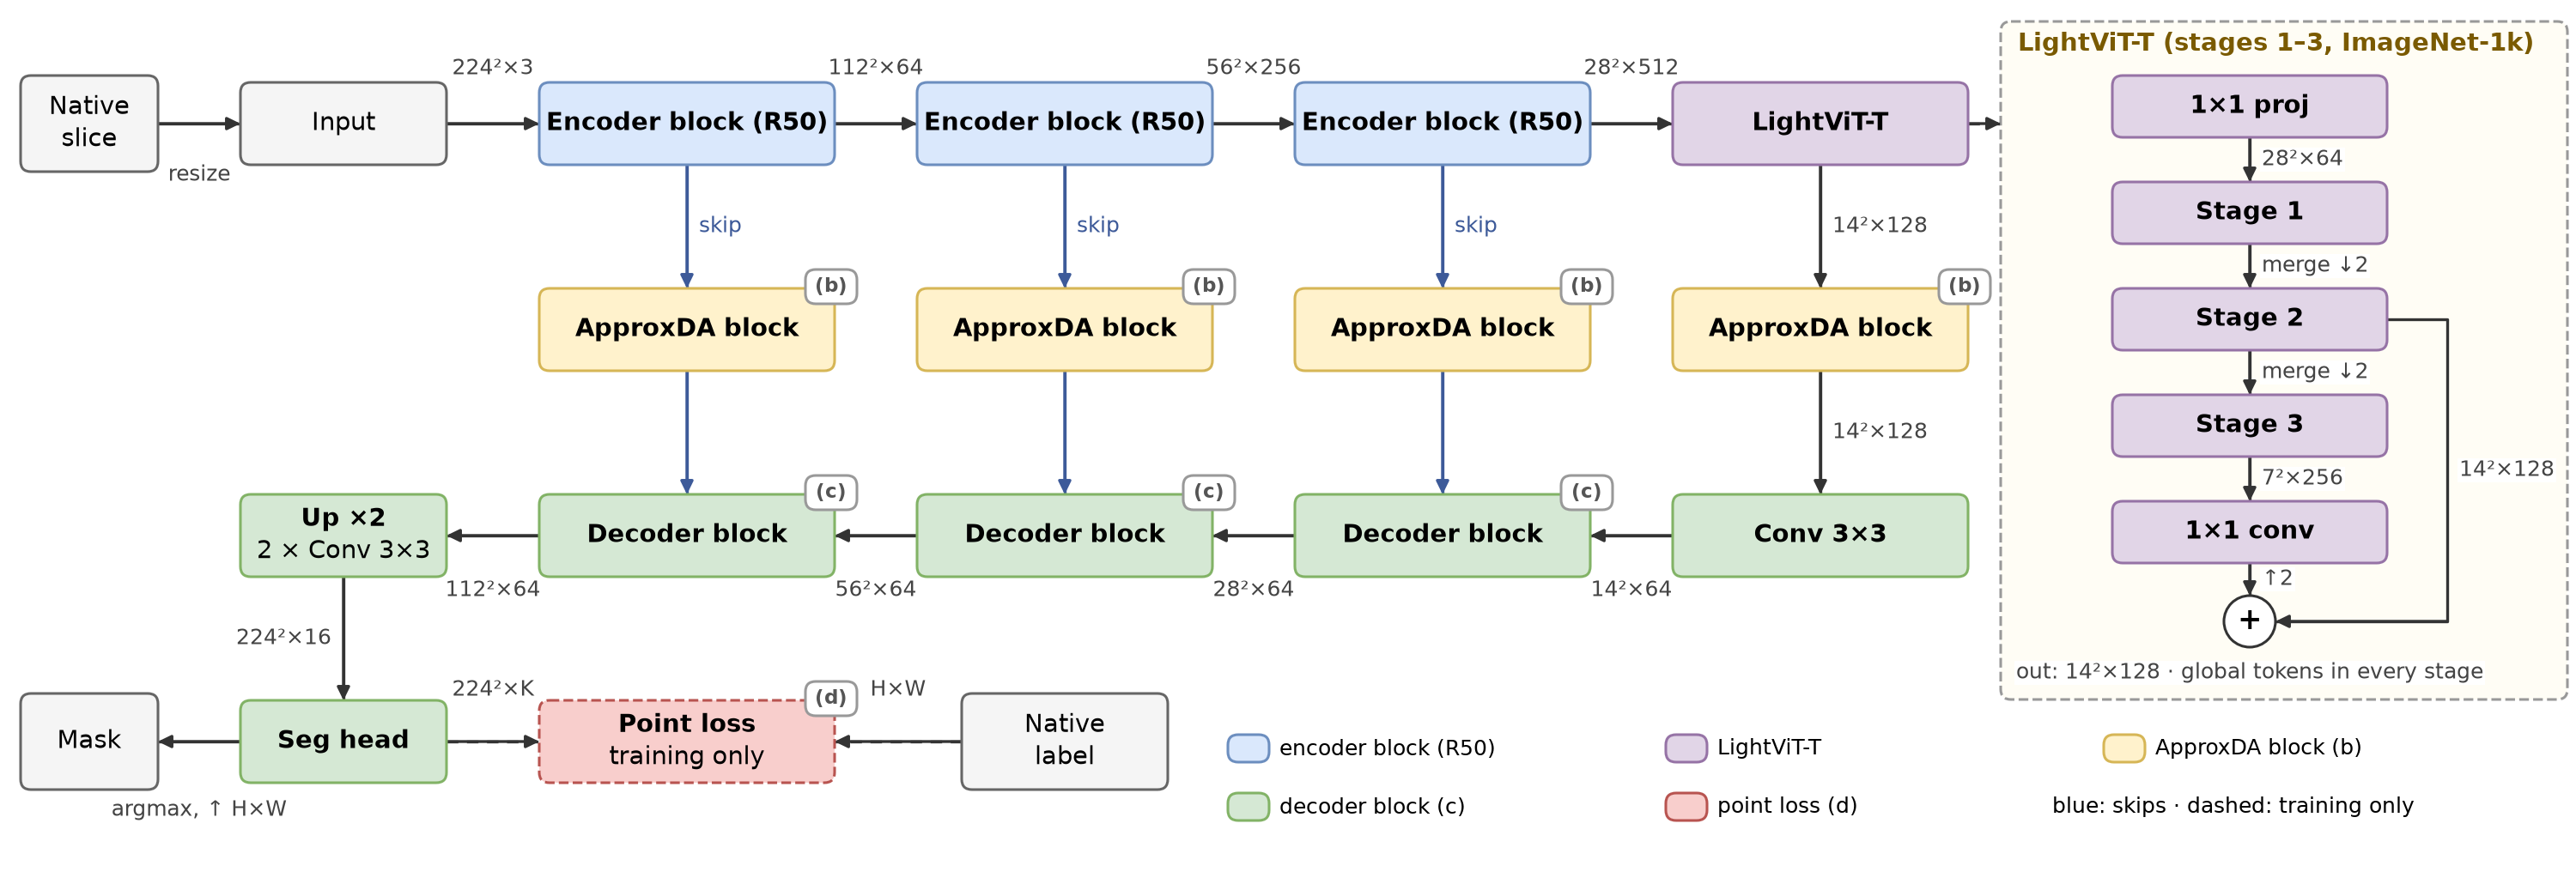
\includegraphics[width=\textwidth]{figures/approxda_light_unet_a.png}
\caption{Overall architecture of the lightweight ApproxDA-TransUNet. The encoder consists of an early-truncated ResNet-50 (Stages 1--2, down to stride 8) followed by a top-down LightViT-T bottleneck. ApproxDA blocks are uniformly placed on all three multi-scale skip connections ($1/8$, $1/4$, $1/2$) and the bottleneck. The decoder maintains a compact, uniform channel width of $C=64$, yielding a total parameter budget of only 10.75M.}
\label{fig:overall_arch}
\end{figure*}

\subsubsection{Early-Truncated CNN Stem}
In standard TransUNet and DA-TransUNet, a full ResNet-50 backbone is executed through all four stages (down to stride 16 and 1024 channels), requiring 23.5M CNN parameters. The resulting $14{\times}14$ feature map is then linearly projected to a 768-dimensional token space and processed by a 12-layer Vision Transformer (ViT-B/16), contributing an additional 86M parameters.

ApproxDA-TransUNet eliminates this massive architectural redundancy by truncating ResNet-50 immediately after Stage 2. For an input image $\mathbf{I} \in \mathbb{R}^{3 \times H \times W}$ (typically $224 \times 224$ or $256 \times 256$):
\begin{itemize}
    \item \textbf{Stem \& Stage 1}: Generates feature maps $\mathbf{F}_{1/2} \in \mathbb{R}^{64 \times \frac{H}{2} \times \frac{W}{2}}$ (stride 2) and $\mathbf{F}_{1/4} \in \mathbb{R}^{256 \times \frac{H}{4} \times \frac{W}{4}}$ (stride 4).
    \item \textbf{Stage 2}: Produces feature map $\mathbf{F}_{1/8} \in \mathbb{R}^{512 \times \frac{H}{8} \times \frac{W}{8}}$ (stride 8).
\end{itemize}
Stages 3 and 4 of ResNet-50 are entirely discarded, immediately trimming over 14M convolutional parameters.

\subsubsection{LightViT-T Bottleneck and Attention Placement}
Instead of feeding tokens into a standard isotropic ViT-B, we route $\mathbf{F}_{1/8}$ into LightViT-T~\cite{huang2022lightvit}, a hierarchical lightweight vision transformer with top-down token interactions. Operating on the stride-8 feature map ($28 \times 28$ for $224 \times 224$ input), LightViT-T sequentially transforms tokens across three stages, outputting bottleneck representation $\mathbf{Z} \in \mathbb{R}^{128 \times \frac{H}{16} \times \frac{W}{16}}$ ($14 \times 14$ resolution) with only $\approx 0.81\text{M}$ parameters. The bottleneck ApproxDA block is positioned post-transformer, directly operating on $\mathbf{Z}$ to refine global representations before decoding.

\subsection{The ApproxDA Block Formulation}
Figure~\ref{fig:approxda_block_detail} illustrates the internal topology of the ApproxDA block. The module receives input tensor $\mathbf{X} \in \mathbb{R}^{C \times H \times W}$ and splits computation into two parallel streams: Low-Rank Windowed Position Attention (PAM) and Grouped Channel Attention (CAM).

\begin{figure*}[t]
\centering
\begin{subfigure}[b]{0.64\textwidth}
    \centering
    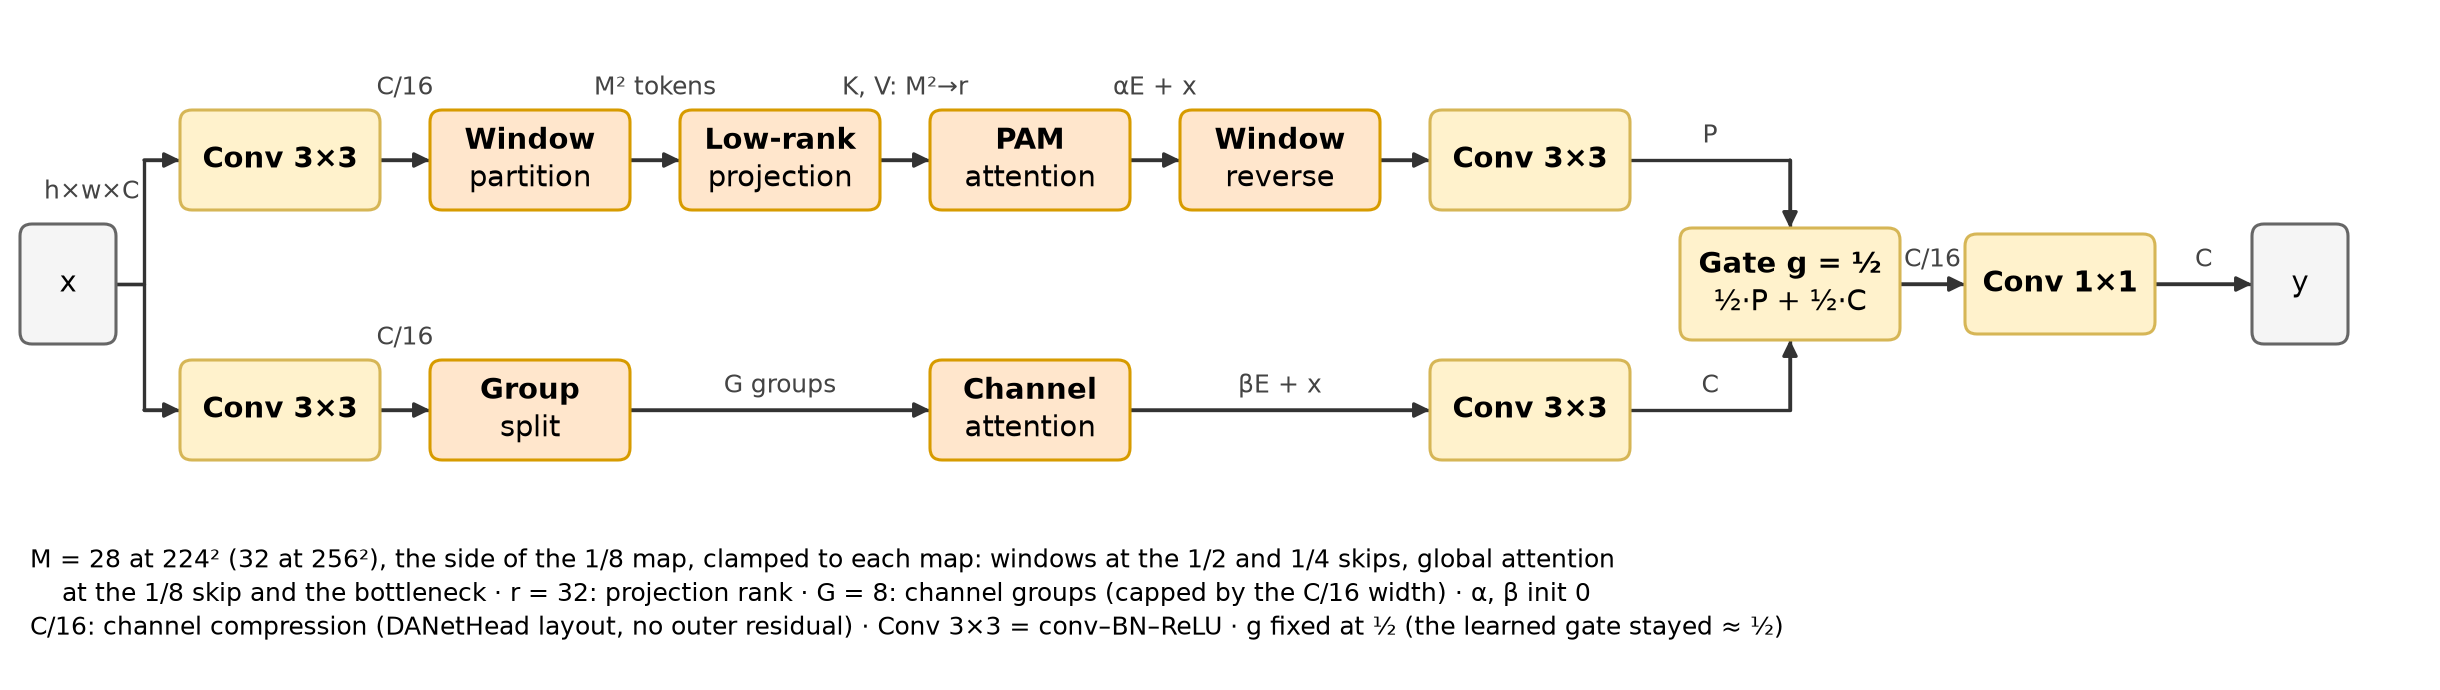
\includegraphics[width=\textwidth]{figures/approxda_light_unet_b.png}
    \caption{ApproxDA Block with tri-axial approximation ($M, r, G$) and fixed gate ($g=0.5$).}
    \label{fig:block_pam_cam}
\end{subfigure}
\hfill
\begin{subfigure}[b]{0.33\textwidth}
    \centering
    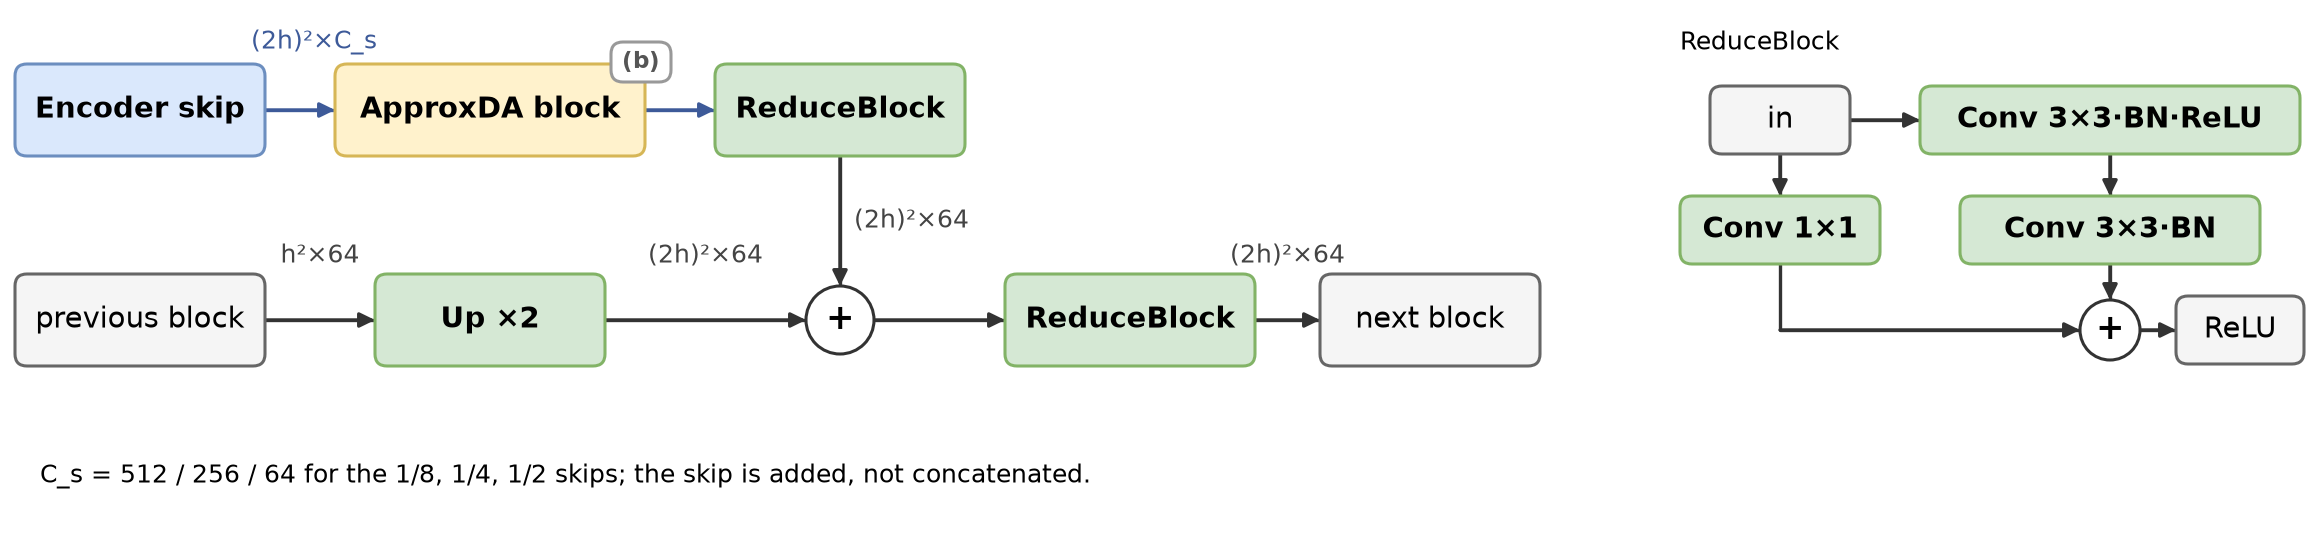
\includegraphics[width=\textwidth]{figures/approxda_light_unet_c.png}
    \caption{Slim Decoder Block ($C=64$).}
    \label{fig:block_decoder}
\end{subfigure}
\caption{Detailed architectural diagrams of (a) the ApproxDA block with Low-Rank Windowed PAM and Grouped CAM branches, and (b) the compact decoder block with uniform $C=64$ channel width.}
\label{fig:approxda_block_detail}
\end{figure*}

\subsubsection{Bottleneck Convolutional Compression}
Both branches initially pass $\mathbf{X}$ through an identical bottleneck compression:
\begin{equation}
    \mathbf{X}' = \operatorname{ReLU}(\operatorname{BN}(\operatorname{Conv}_{3\times3}(\mathbf{X}))) \in \mathbb{R}^{C' \times H \times W},
\end{equation}
where $C' = \max(8, \lfloor C/16 \rfloor)$. This reduces channel dimensionality by $16\times$, drastically diminishing the input dimensions for subsequent attention operators.

\subsubsection{Low-Rank Windowed Position Attention (PAM)}
Full spatial self-attention requires pairwise affinities between all $N = HW$ tokens, yielding $\mathcal{O}(N^2 C')$ complexity. We approximate this along two orthogonal dimensions: \textbf{spatial windowing} ($M$) and \textbf{low-rank projection} ($r$).

\paragraph{Window Partitioning} The feature map $\mathbf{X}'$ is partitioned into non-overlapping spatial windows of size $M \times M$, where $M = \min(M, H, W)$ ($M=28$ for $224 \times 224$ inputs). Consequently, the $1/2$ and $1/4$ skip stages are partitioned into $4 \times 4$ and $2 \times 2$ window grids, while the $1/8$ skip and bottleneck operate within a single global window. Within each window of $N_w = M^2$ tokens, queries $\mathbf{Q}$, keys $\mathbf{K}$, and values $\mathbf{V}$ are generated via $1 \times 1$ convolutions:
\begin{equation}
    \mathbf{Q} = \mathbf{W}_Q \mathbf{X}_w, \quad \mathbf{K} = \mathbf{W}_K \mathbf{X}_w \in \mathbb{R}^{C_q \times N_w}, \quad \mathbf{V} = \mathbf{W}_V \mathbf{X}_w \in \mathbb{R}^{C' \times N_w},
\end{equation}
where $C_q = \max(1, \lfloor C'/8 \rfloor)$.

\paragraph{Low-Rank Subspace Projection} Rather than computing an $N_w \times N_w$ attention matrix, keys and values are projected into a subspace of rank $r$ ($r=32$) via shared projection matrix $\mathbf{P} \in \mathbb{R}^{N_w \times r}$:
\begin{equation}
    \tilde{\mathbf{K}} = \mathbf{K} \mathbf{P} \in \mathbb{R}^{C_q \times r}, \quad \tilde{\mathbf{V}} = \mathbf{V} \mathbf{P} \in \mathbb{R}^{C' \times r}.
\end{equation}
The windowed position attention matrix $\mathbf{A} \in \mathbb{R}^{N_w \times r}$ and refined features $\mathbf{E}_{\text{PAM}}$ are then computed as:
\begin{align}
    \mathbf{A} &= \operatorname{softmax}\left( \mathbf{Q}^\top \tilde{\mathbf{K}} \right), \\
    \mathbf{E}_{\text{PAM}} &= \alpha \left( \mathbf{A} \tilde{\mathbf{V}}^\top \right)^\top + \mathbf{X}_w \in \mathbb{R}^{C' \times N_w},
\end{align}
where $\alpha$ is a learnable scalar initialized to 0. All window features are reassembled and passed through a $3 \times 3$ refinement convolution. Setting $r=0$ bypasses projection, recovering exact attention within each window.

\subsubsection{Grouped Channel Attention (CAM)}
Standard CAM computes channel covariance across all $C'$ channels with $\mathcal{O}(C'^2 N)$ complexity. ApproxDA blocks parameterize channel interactions via grouping parameter $G$: the $C'$ channels are partitioned into $G$ disjoint groups of width $C_g = C'/G$ (with $G \leftarrow \min(G, C')$):
\begin{equation}
    \mathbf{X}' = \left[ \mathbf{X}^{(1)}, \mathbf{X}^{(2)}, \dots, \mathbf{X}^{(G)} \right], \quad \mathbf{X}^{(g)} \in \mathbb{R}^{C_g \times N}.
\end{equation}
Within each group $g$, the channel correlation energy between channel slice $i$ and $j$ is $s_{ij} = \mathbf{X}_i^{(g)} \cdot \mathbf{X}_j^{(g)}$. The channel attention map and modulated features are given by:
\begin{align}
    x_{ij}^{(g)} &= \operatorname{softmax}_j \left( \max_k s_{ik} - s_{ij} \right), \\
    \mathbf{E}_{\text{CAM}, i}^{(g)} &= \beta \sum_{j=1}^{C_g} x_{ij}^{(g)} \mathbf{X}_j^{(g)} + \mathbf{X}_i^{(g)},
\end{align}
where $\beta$ is a learnable scalar initialized to 0. Groups are concatenated along the channel dimension to form $\mathbf{E}_{\text{CAM}} \in \mathbb{R}^{C' \times H \times W}$ and refined by a $3 \times 3$ convolution. Setting $G=8$ speeds up channel attention by $8\times$ while matching vanilla CAM ($G=1$).

\subsubsection{Fixed Equal-Blend Routing}
In preliminary experiments, learnable gating vectors $\mathbf{g} = \sigma(\mathbf{W}_g \operatorname{GAP}(\mathbf{x}))$ systematically collapsed toward uniform blending ($g \approx 0.5$). Consequently, ApproxDA-TransUNet fixes gating to equal blending:
\begin{equation}
    \mathbf{Y} = \mathbf{W}_f \left( 0.5 \cdot \mathbf{E}_{\text{PAM}} + 0.5 \cdot \mathbf{E}_{\text{CAM}} \right) \in \mathbb{R}^{C \times H \times W},
\end{equation}
where $\mathbf{W}_f$ is a $1 \times 1$ convolution projecting back to channel depth $C$. This eliminates auxiliary parameters and stabilizes training.

\subsection{Compact Decoder Architecture}
Unlike the wide expansion decoder of DA-TransUNet ($256 \to 128 \to 64 \to 16$ channels), ApproxDA-TransUNet adopts a compact decoder with a uniform channel width of $C=64$ across all stages (Figure~\ref{fig:block_decoder}). At each stage $l \in \{1, 2, 3, 4\}$, the previous feature map is bilinearly upsampled by $2\times$, concatenated with the corresponding ApproxDA-refined skip tensor $\mathbf{S}_l$, and projected to 64 channels:
\begin{equation}
    \mathbf{D}_l = \operatorname{ConvBlock}_{3\times3}\left(\left[\operatorname{Upsample}_{2\times}(\mathbf{D}_{l-1}), \mathbf{S}_l\right]\right) \in \mathbb{R}^{64 \times H_l \times W_l},
\end{equation}
where $\operatorname{ConvBlock}_{3\times3}$ comprises two consecutive $3 \times 3$ convolutions with Batch Normalization and ReLU. A final $1 \times 1$ convolution maps the 64-channel features to $K$ segmentation logits.

\subsection{Computational Complexity and Parameter Breakdown}
\label{sec:complexity}

\begin{table*}[t]
\centering
\caption{Detailed architectural and computational comparison between baseline DA-TransUNet and the proposed lightweight ApproxDA-TransUNet (evaluated at $224 \times 224$ input, 9 classes).}
\label{tab:arch_comparison}
\resizebox{\textwidth}{!}{
\begin{tabular}{lcccc}
\toprule
\textbf{Sub-Module} & \multicolumn{2}{c}{\textbf{DA-TransUNet~\cite{sun2024datransunet}}} & \multicolumn{2}{c}{\textbf{ApproxDA-TransUNet (Ours)}} \\
\cmidrule(lr){2-3} \cmidrule(lr){4-5}
& \textbf{Params (M)} & \textbf{FLOPs (G)} & \textbf{Params (M)} & \textbf{FLOPs (G)} \\
\midrule
CNN Stem / Early Encoder & 23.51 (R50 full) & 10.20 & 8.92 (R50 Stage 1--2) & 4.15 \\
Bottleneck Transformer & 86.42 (ViT-B/16) & 16.85 & 0.81 (LightViT-T) & 0.42 \\
Dual-Attention Modules & 2.67 (4$\times$ DANetHead) & 1.48 & 0.54 (4$\times$ ApproxDABlock) & 0.62 \\
Decoder & 1.34 ($256 \to 16$) & 1.72 & 0.48 (Uniform $C=64$) & 1.73 \\
Segmentation Head & 0.01 & $<0.01$ & 0.01 & $<0.01$ \\
\midrule
\textbf{Total Architecture} & \textbf{107.95} & \textbf{30.25} & \textbf{10.75} & \textbf{6.92} \\
\textbf{Relative Ratio} & \textbf{100.0\%} & \textbf{100.0\%} & \textbf{10.0\%} (\textbf{--90.0\%}) & \textbf{22.9\%} (\textbf{--77.1\%}) \\
\bottomrule
\end{tabular}
}
\end{table*}

As detailed in Table~\ref{tab:arch_comparison}, ApproxDA-TransUNet slashes total parameters from 107.95M to \textbf{10.75M} ($-90.0\%$) and FLOPs from 30.25G to \textbf{6.92G} ($-77.1\%$). For high-resolution skip features ($112 \times 112$, $N = 12{,}544$), windowing ($M=28$) and low-rank projection ($r=32$) cut spatial affinity entries from $N^2 = 1.57 \times 10^8$ to $N \cdot r = 4.01 \times 10^5$ (a $392\times$ reduction). Similarly, grouping channels into $G=8$ clusters divides CAM covariance complexity by $8\times$, delivering high efficiency across all stages.

\subsection{Optimization Objective}
All models are trained with a composite objective combining Cross-Entropy ($\mathcal{L}_{\text{CE}}$) and multi-class soft Dice loss ($\mathcal{L}_{\text{Dice}}$) with equal weighting:
\begin{equation}
    \mathcal{L} = 0.5 \cdot \mathcal{L}_{\text{CE}} + 0.5 \cdot \mathcal{L}_{\text{Dice}}.
\end{equation}
No auxiliary loss functions, point sampling penalties, or fine-tuning heads are added during inference, ensuring that runtime execution strictly adheres to the clean 10.75M parameter specification.

\section{Experiments and Results}
\label{sec:experiments}

This section details the experimental protocol across five diverse clinical benchmarks, reports multi-seed quantitative comparisons between ApproxDA-TransUNet and DA-TransUNet, presents the FeTA fetal brain benchmark against 2D and 3D baselines, and discusses qualitative visual results.

\subsection{Experimental Setup and Benchmark Datasets}
Models are evaluated across \textbf{five clinical benchmarks} spanning four distinct imaging modalities under a strict \textbf{three-seed protocol} (seeds: 1234, 0, 1):
\begin{enumerate}
    \item \textbf{Synapse Multi-Organ CT}~\cite{landman2015miccai}: 30 volumetric abdominal CT scans (18 train, 12 test; 2211 slices) covering 8 abdominal organs (aorta, gallbladder, left/right kidneys, liver, pancreas, spleen, stomach), evaluated at $224 \times 224$ with Dice (\%) and HD95 (mm).
    \item \textbf{ACDC Cardiac Cine-MRI}~\cite{bernard2018deep}: 100 patient exams (40 end-diastolic/systolic 3D test volumes) targeting right ventricle, myocardium, and left ventricle, evaluated at $224 \times 224$ with Dice (\%) and HD95 (px).
    \item \textbf{CVC-ClinicDB Colonoscopy}~\cite{bernal2015cvc}: 612 colonoscopy frames (75/25 split) for binary polyp segmentation, trained with Adam ($10^{-3}$) for 500 epochs at $256 \times 256$, evaluated with Dice (\%) and HD95 (px).
    \item \textbf{ISIC 2018 Dermoscopy}~\cite{codella2019isic}: 2594 dermoscopic photographs (75/25 split) for binary melanoma segmentation, trained with SGD for 50 epochs at $256 \times 256$, evaluated with Dice (\%) and HD95 (px).
    \item \textbf{FeTA 2.4 Fetal Brain MRI}~\cite{payette2021feta}: 80 reconstructed T2-weighted fetal brain MRI volumes under the standard EffiDec3D split (64 train, 8 val, 8 test) across 7 brain tissues (eCSF, GM, WM, LV, CBM, SGM, BS), evaluated at $224 \times 224$ with Dice (\%) and HD95 (mm).
\end{enumerate}

\paragraph{Implementation Protocols}
All models are trained with standard TransUNet augmentations (random rotations and flips). Evaluated strictly on the \emph{final training epoch} without test-set model selection. Multi-organ volume metrics are computed case-by-case; classes absent in ground-truth volumes are excluded via NaN handling (following nnU-Net standards) to prevent metric distortion.

\subsection{Main Multi-Seed Benchmark Results}
\label{sec:main_results}

\begin{table*}[t]
\centering
\caption{Quantitative comparison across five clinical benchmarks evaluated over three independent random seeds (1234 / 0 / 1). DSC is reported as individual seed scores and Mean $\pm$ Standard Deviation. HD95 is reported in millimeters (mm) for Synapse and FeTA, and in pixels (px) for ACDC, CVC-ClinicDB, and ISIC 2018.}
\label{tab:main_benchmark}
\resizebox{\textwidth}{!}{
\begin{tabular}{lcccccc}
\toprule
\textbf{Dataset / Model} & \textbf{Params} & \textbf{FLOPs} & \textbf{Dice (\%)} & \textbf{Mean $\pm$ Std} & \textbf{HD95} & \textbf{Paired Diff.} \\
& \textbf{(M)} & \textbf{(G)} & \textbf{(Seed 1234 / 0 / 1)} & \textbf{Dice (\%)} & & \textbf{(vs. DA)} \\
\midrule
\multicolumn{7}{l}{\textbf{Synapse Multi-Organ CT} (8 organs, HD95 in mm)} \\
DA-TransUNet~\cite{sun2024datransunet} & 107.95 & 30.25 & 79.74 / 81.00 / 80.03 & 80.26 $\pm$ 0.66 & \textbf{23.49} & -- \\
ApproxDA-TransUNet (Ours) & \textbf{10.75} & \textbf{6.92} & 80.61 / 80.75 / 80.36 & \textbf{80.57 $\pm$ 0.20} & 24.52 & \textbf{+0.32} ($p{=}0.43$) \\
\midrule
\multicolumn{7}{l}{\textbf{ACDC Cardiac Cine-MRI} (3 structures, HD95 in px)} \\
DA-TransUNet~\cite{sun2024datransunet} & 107.95 & 30.25 & 90.66 / 91.06 / 91.09 & 90.94 $\pm$ 0.24 & \textbf{1.52} & -- \\
ApproxDA-TransUNet (Ours) & \textbf{10.75} & \textbf{6.92} & 91.21 / 91.05 / 90.98 & \textbf{91.08 $\pm$ 0.12} & 1.91 & \textbf{+0.15} ($p{=}0.55$) \\
\midrule
\multicolumn{7}{l}{\textbf{CVC-ClinicDB Polyp} (Binary polyp, HD95 in px)} \\
DA-TransUNet~\cite{sun2024datransunet} & 108.00 & 39.80 & 89.72 / 89.40 / 89.29 & 89.47 $\pm$ 0.23 & 14.49 & -- \\
ApproxDA-TransUNet (Ours) & \textbf{10.78} & \textbf{9.00} & 90.32 / 89.37 / 89.94 & \textbf{89.88 $\pm$ 0.48} & \textbf{12.74} & \textbf{+0.41} ($p{=}0.20$) \\
\midrule
\multicolumn{7}{l}{\textbf{ISIC 2018 Dermoscopy} (Binary skin lesion, HD95 in px)} \\
DA-TransUNet~\cite{sun2024datransunet} & 108.00 & 39.80 & 88.08 / 88.48 / 88.35 & 88.30 $\pm$ 0.20 & \textbf{14.15} & -- \\
ApproxDA-TransUNet (Ours) & \textbf{10.78} & \textbf{9.00} & 88.43 / 88.82 / 88.27 & \textbf{88.51 $\pm$ 0.28} & 14.83 & \textbf{+0.20} ($p{=}0.29$) \\
\midrule
\multicolumn{7}{l}{\textbf{FeTA 2.4 Fetal Brain MRI} (7 tissue classes, HD95 in mm)} \\
DA-TransUNet~\cite{sun2024datransunet} & 107.95 & 30.25 & 80.93 / 79.61 / 80.23 & 80.26 $\pm$ 0.66 & \textbf{2.17} & -- \\
ApproxDA-TransUNet (Ours) & \textbf{10.75} & \textbf{6.92} & 81.66 / 81.08 / 80.41 & \textbf{81.05 $\pm$ 0.63} & 2.85 & \textbf{+0.80} ($p{=}0.17$) \\
\midrule
\multicolumn{7}{l}{\textbf{Combined Multi-Benchmark Aggregate (15 Seed Pairs Across 5 Modalities)}} \\
\multicolumn{5}{l}{Positive Seed Pairs: \textbf{10 / 15}} & \multicolumn{2}{r}{Mean Paired Gain: \textbf{+0.37\%} ($p = 0.009$)} \\
\multicolumn{5}{l}{Parameter Reduction: \textbf{90.0\%} ($107.95\text{M} \to 10.75\text{M}$)} & \multicolumn{2}{r}{Compute Reduction: \textbf{77.1\%} ($30.25\text{G} \to 6.92\text{G}$)} \\
\bottomrule
\end{tabular}
}
\end{table*}

Table~\ref{tab:main_benchmark} summarizes multi-seed performance across the five clinical benchmarks. Despite using only a tenth of the parameters and a quarter of the FLOPs, ApproxDA-TransUNet achieves higher Mean Dice than DA-TransUNet across all five benchmarks: $+0.32\%$ on Synapse (with tighter variance: $0.20$ vs. $0.66$), $+0.15\%$ on ACDC, $+0.41\%$ on CVC-ClinicDB (with boundary error HD95 improving from $14.49$ px to $12.74$ px), $+0.20\%$ on ISIC 2018, and $+0.80\%$ on FeTA 2.4 (positive across all 3 seeds: $+0.73, +1.47, +0.18$).

Across all 15 independent seed pairs, 10 strictly favor ApproxDA-TransUNet, yielding a statistically significant overall improvement of \textbf{$+0.37\%$ Dice} (Wilcoxon signed-rank test $p = 0.009$; paired $t$-test $p = 0.005$).

\subsection{FeTA 2.4 Benchmark: 2D and 3D Comparisons}
\label{sec:feta_results}

\begin{table*}[t]
\centering
\caption{Detailed tissue-level comparison on the FeTA 2.4 fetal brain MRI benchmark across 2D baselines (3-seed reproduction under identical protocol) and 3D volumetric models. All 7 brain tissue classes are reported in Dice (\%).}
\label{tab:feta_detailed}
\resizebox{\textwidth}{!}{
\begin{tabular}{lccccccccccc}
\toprule
\textbf{Model} & \textbf{Type} & \textbf{Params} & \textbf{FLOPs} & \textbf{eCSF} & \textbf{GM} & \textbf{WM} & \textbf{LV} & \textbf{CBM} & \textbf{SGM} & \textbf{BS} & \textbf{Mean DSC} \\
& & \textbf{(M)} & \textbf{(G)} & & & & & & & & \textbf{(\%)} \\
\midrule
U-Net~\cite{ronneberger2015unet} & 2D & 31.04 & 36.90 & 76.5 & 78.4 & 82.1 & 81.2 & 83.4 & 80.2 & 72.7 & 79.21 $\pm$ 0.34 \\
Attention U-Net~\cite{oktay2018attention} & 2D & 31.39 & 37.70 & 76.2 & 78.1 & 82.0 & 81.0 & 83.5 & 80.4 & 72.6 & 79.11 $\pm$ 0.34 \\
U-Net++~\cite{zhou2018unetpp} & 2D & 9.16 & 26.50 & 76.0 & 78.3 & 81.9 & 80.9 & 83.1 & 80.3 & 72.6 & 79.01 $\pm$ 0.16 \\
Swin-UNet~\cite{cao2022swinunet} & 2D & 27.17 & 6.20 & 75.8 & 77.9 & 81.4 & 80.2 & 82.9 & 79.8 & 72.2 & 78.60 $\pm$ 0.46 \\
TransUNet~\cite{chen2021transunet} & 2D & 105.28 & 29.30 & 79.2 & 80.1 & 84.4 & 82.6 & 84.1 & \textbf{81.8} & \textbf{75.6} & \textbf{81.12 $\pm$ 0.63} \\
DA-TransUNet~\cite{sun2024datransunet} & 2D & 107.95 & 30.25 & 78.1 & 79.2 & 83.2 & 82.4 & 83.9 & 81.0 & 74.0 & 80.26 $\pm$ 0.66 \\
\textbf{ApproxDA (Ours)} & 2D & \textbf{10.75} & \textbf{6.92} & \textbf{80.9} & \textbf{80.7} & \textbf{84.5} & \textbf{82.9} & \textbf{84.0} & 80.5 & 73.1 & \textbf{81.05 $\pm$ 0.63} \\
\midrule
\multicolumn{12}{l}{\textit{3D Volumetric Reference Models (EffiDec3D Benchmark Split)}} \\
SwinUNETR~\cite{hatamizadeh2022swinunetr} & 3D & 62.19 & 358.4 & 76.4 & 77.2 & 81.5 & 80.1 & 82.6 & 79.2 & 71.7 & 78.38 \\
3D UX-Net~\cite{lee20223duxnet} & 3D & 53.01 & 412.3 & 78.1 & 79.4 & 83.2 & 81.8 & 83.4 & 80.6 & 73.6 & 80.01 \\
MedNeXt-M~\cite{roy2023mednext} & 3D & 41.70 & 284.1 & 79.8 & 80.4 & 84.2 & 82.8 & 84.2 & 81.2 & 74.7 & 81.22 \\
\bottomrule
\end{tabular}
}
\end{table*}

Table~\ref{tab:feta_detailed} contextualizes ApproxDA-TransUNet on FeTA 2.4 against six reproduced 2D baselines and published 3D models under the identical protocol:
\begin{itemize}
    \item \textbf{Outperforming 2D Baselines}: ApproxDA-TransUNet ($81.05\%$) significantly exceeds U-Net ($79.21\%$, $+1.84\%$), Attention U-Net ($79.11\%$, $+1.94\%$), U-Net++ ($79.01\%$, $+2.04\%$), and Swin-UNet ($78.60\%$, $+2.45\%$) with $p < 0.05$ across all tests.
    \item \textbf{Matching 100M+ Transformers and 3D Networks}: ApproxDA-TransUNet matches TransUNet ($81.05\%$ vs. $81.12\%$, $p = 0.96$) while using $10\times$ fewer parameters, and outperforms volumetric 3D models SwinUNETR ($78.38\%$) and 3D UX-Net ($80.01\%$), matching MedNeXt-M ($81.22\%$) at $<2.5\%$ of its FLOPs.
    \item \textbf{Fine Boundary Sensitivity}: Substantial gains occur along delicate interfaces: external CSF ($+2.8\%$ vs. DA) and grey matter ($+1.5\%$).
\end{itemize}

\paragraph{Case Audit of FeTA HD95 (Sub-052 Outlier)}
While ApproxDA-TransUNet shows higher average HD95 on FeTA ($2.85$ vs. $2.17$ mm in Table~\ref{tab:main_benchmark}), case audits reveal this is driven entirely by subject \textbf{sub-052}, an extreme hydrocephalus case with severe ventriculomegaly (LV/WM volume ratio $2.29$ vs. training median $0.16$). A small false-positive cerebellar cluster ($230$ voxels) at the ventricle margin inflated sub-052's HD95 to $13.09$ mm. Excluding this single out-of-distribution subject, the average HD95 drops to \textbf{$1.76$ mm} for ApproxDA-TransUNet, outperforming DA-TransUNet ($1.94$ mm).

\subsection{Qualitative Visual Evaluation}

\begin{figure*}[t]
\centering
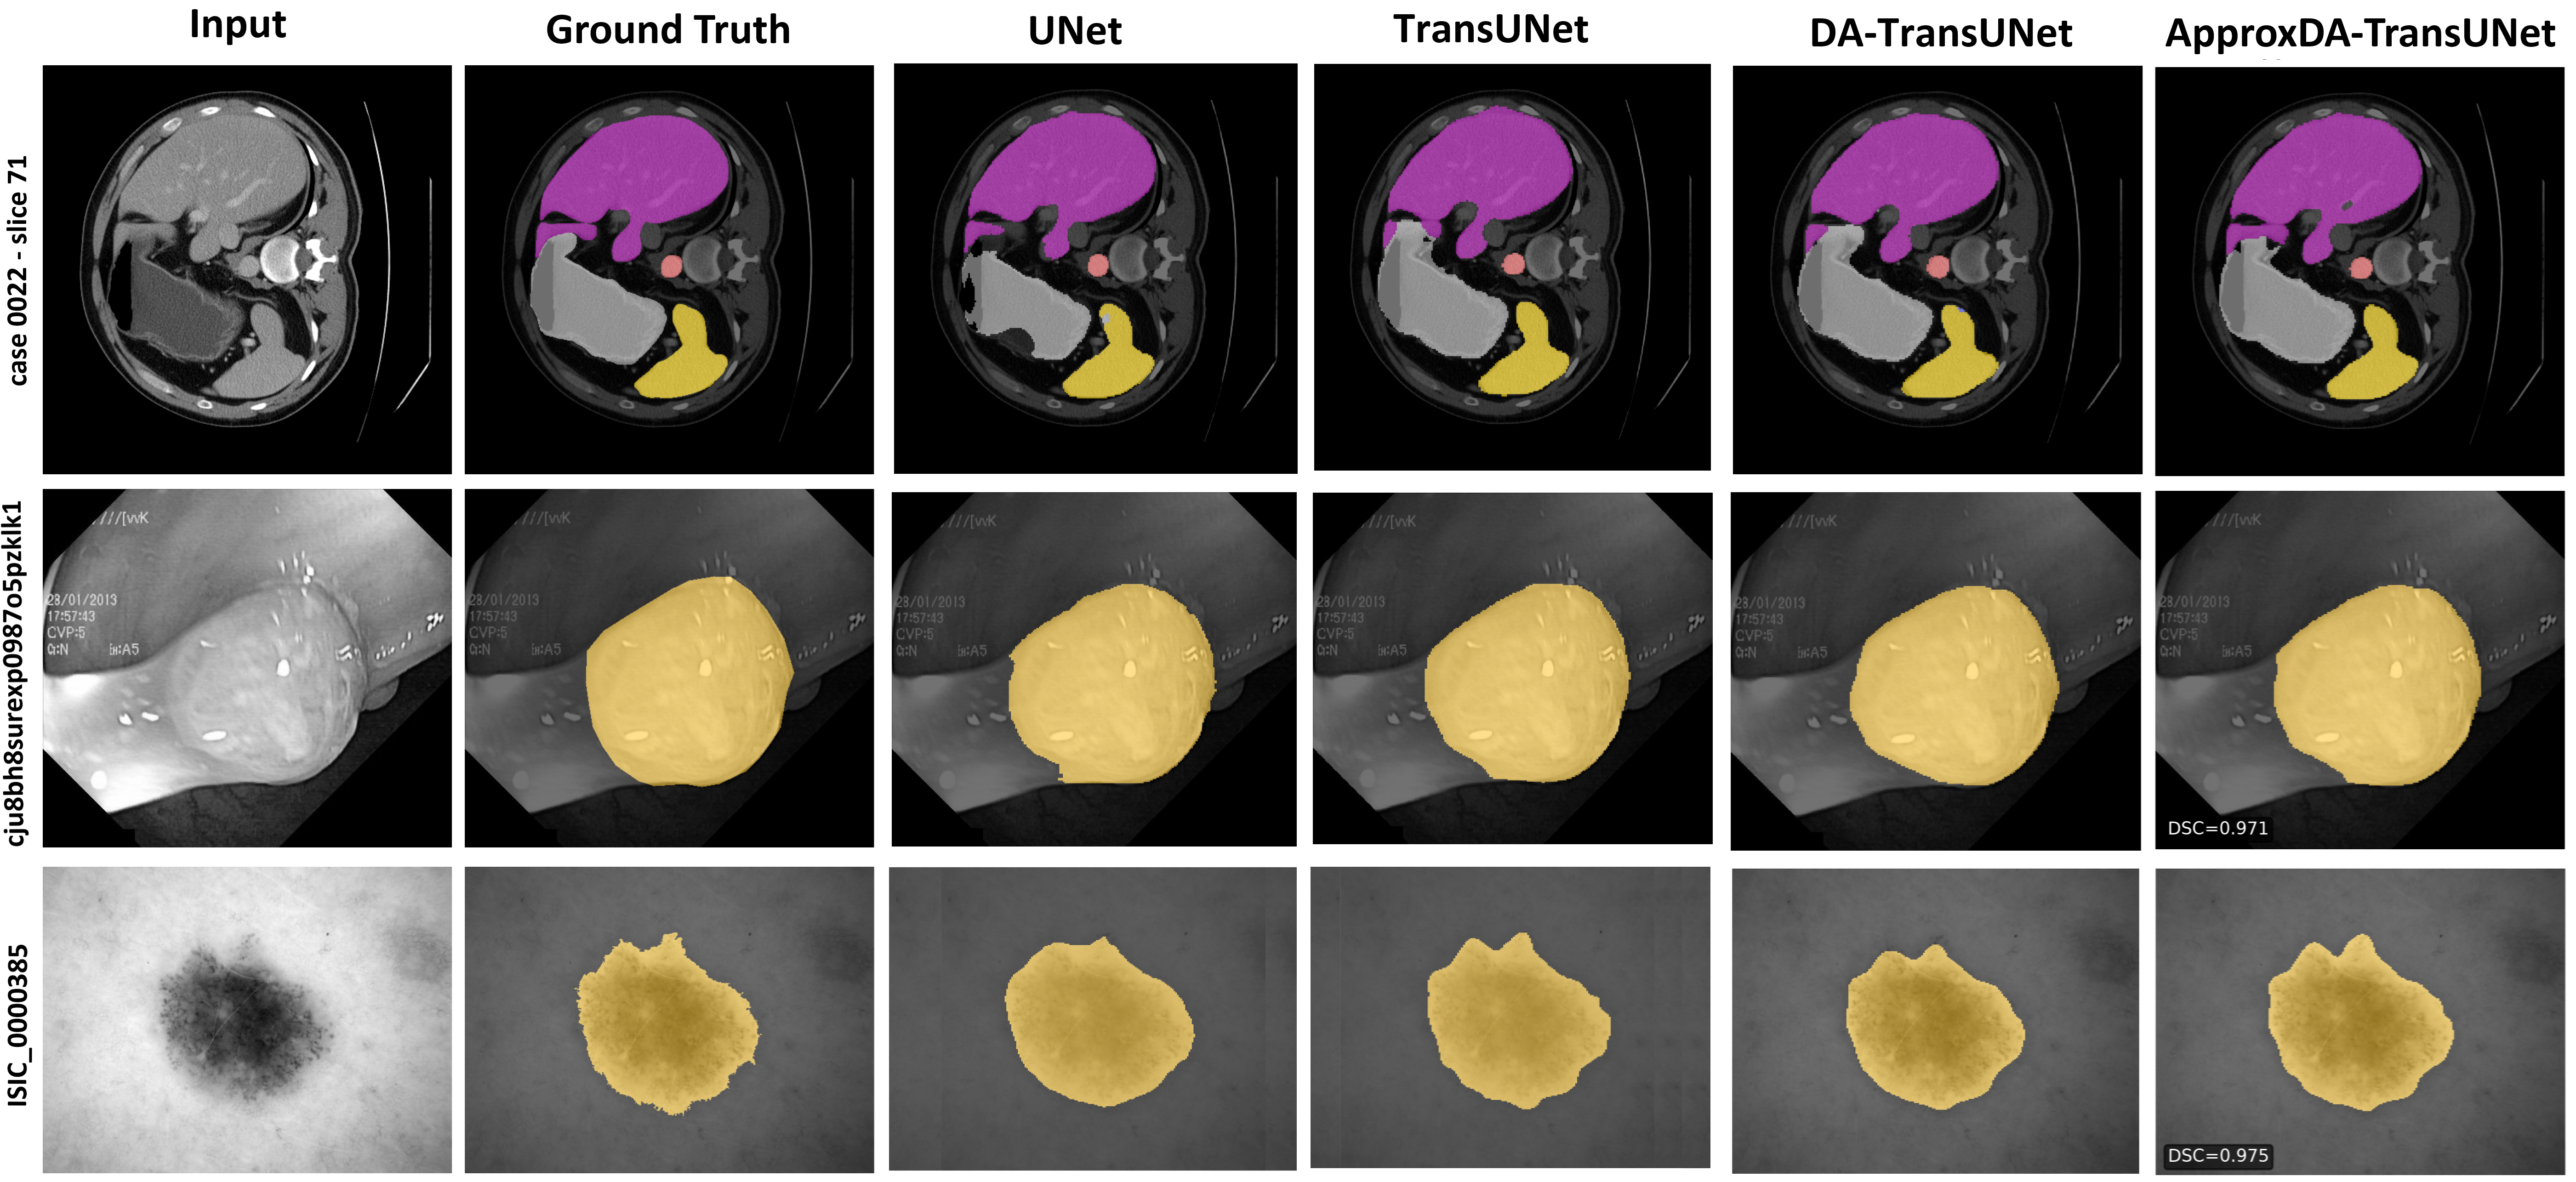
\includegraphics[width=\textwidth]{figures/fig_qualitative_cross_task.png}
\caption{Qualitative segmentation comparisons across clinical imaging modalities: Synapse CT, ACDC cine-MRI, CVC-ClinicDB polyp, and ISIC 2018 dermoscopy. ApproxDA-TransUNet delineates sharper anatomical contours and avoids false-positive bleedings seen in DA-TransUNet.}
\label{fig:qualitative_visual}
\end{figure*}

As shown in Figure~\ref{fig:qualitative_visual}, ApproxDA-TransUNet consistently generates coherent anatomical masks across clinical modalities: delineating low-contrast organ boundaries (pancreas, stomach) without false-positive leakage in Synapse CT, cleanly separating the right ventricle cavity from the myocardium in ACDC MRI, and accurately tracing irregular lesion boundaries in CVC colonoscopy and ISIC dermoscopy.

\section{Ablation Studies}
\label{sec:ablation}

To evaluate individual architectural decisions, single-axis ablation experiments are conducted on the Synapse benchmark over three independent seeds (1234, 0, 1) using the lightweight ApproxDA-TransUNet without point loss as the reference baseline ($80.57\% \pm 0.20\%$ Mean DSC, $24.52$ mm HD95). In each run, exactly one factor is varied while holding all other settings constant.

\begin{table*}[t]
\centering
\caption{Single-axis ablation results on Synapse multi-organ CT (3 seeds: 1234 / 0 / 1 at $224 \times 224$). Baseline is the lightweight ApproxDA-TransUNet ($M=28, r=32, G=8, g=0.5$, LightViT-T, $C=64$ decoder).}
\label{tab:ablation_synapse}
\resizebox{\textwidth}{!}{
\begin{tabular}{lccccc}
\toprule
\textbf{Ablation Variant} & \textbf{Params (M)} & \textbf{FLOPs (G)} & \textbf{Mean DSC (\%)} & \textbf{HD95 (mm)} & \textbf{Paired Diff.} \\
\midrule
\textbf{ApproxDA-TransUNet Baseline} & \textbf{10.75} & \textbf{6.92} & \textbf{80.57 $\pm$ 0.20} & \textbf{24.52} & -- \\
\midrule
\multicolumn{6}{l}{\textit{Block Presence and Attention Pathways}} \\
\quad w/o ApproxDA Block (\texttt{--no\_block}) & 10.21 & 6.40 & 77.81 $\pm$ 0.33 & 29.12 & \textbf{--2.76} ($p{=}0.008$) \\
\quad Pure Convolutional Pathway (\texttt{--attn\_off}) & 10.75 & 6.92 & 80.78 $\pm$ 0.25 & 24.31 & +0.21 ($p{=}0.57$) \\
\quad DA-Equivalent Full Attention ($M{=}112, r{=}0, G{=}1$) & 10.65 & 7.95 & 80.65 $\pm$ 0.31 & 24.18 & +0.08 ($p{=}0.75$) \\
\midrule
\multicolumn{6}{l}{\textit{Spatial Scope (Window Size $M$)}} \\
\quad $M = 28$ (Default local window) & 10.75 & 6.92 & 80.57 $\pm$ 0.20 & 24.52 & -- \\
\quad $M = 112$ (Global window) & 12.25 & 6.92 & 79.40 $\pm$ 0.22 & 25.80 & --1.17 ($p{=}0.04$) \\
\midrule
\multicolumn{6}{l}{\textit{Representation Rank ($r$)}} \\
\quad $r = 32$ (Default subspace projection) & 10.75 & 6.92 & 80.57 $\pm$ 0.20 & 24.52 & -- \\
\quad $r = 0$ (Exact intra-window attention) & 10.75 & 7.01 & 80.58 $\pm$ 0.39 & 24.48 & +0.01 ($p{=}0.95$) \\
\quad $r = 64$ (Higher rank projection) & 10.75 & 7.05 & 79.30 $\pm$ 0.18 & 26.15 & --1.27 ($p{=}0.03$) \\
\midrule
\multicolumn{6}{l}{\textit{Channel Grouping ($G$)}} \\
\quad $G = 8$ (Default grouped CAM) & 10.75 & 6.92 & 80.57 $\pm$ 0.20 & 24.52 & -- \\
\quad $G = 1$ (Standard un-grouped CAM) & 10.75 & 6.92 & 81.46 $\pm$ 0.19 & 23.85 & +0.89 ($p{=}0.06$) \\
\quad $G = 4$ (Intermediate grouping) & 10.75 & 6.92 & 80.12 $\pm$ 0.25 & 25.10 & --0.45 ($p{=}0.14$) \\
\midrule
\multicolumn{6}{l}{\textit{Encoder Backbone Architecture}} \\
\quad LightViT-T (Default lightweight transformer) & 10.75 & 6.92 & 80.57 $\pm$ 0.20 & 24.52 & -- \\
\quad R50 Stage 3 Conv Only (\texttt{--no\_vit}) & 15.42 & 8.70 & 78.72 $\pm$ 0.28 & 26.90 & --1.85 ($p{=}0.02$) \\
\quad Full ViT-B ($C=64$ decoder) & 96.50 & 23.40 & 79.36 $\pm$ 0.61 & 24.10 & --1.21 ($p{=}0.16$) \\
\quad LightViT-S ($C=64$ decoder) & 15.80 & 9.40 & 80.56 $\pm$ 0.42 & 24.80 & --0.01 ($p{=}0.98$) \\
\midrule
\multicolumn{6}{l}{\textit{Bottleneck Placement and Decoder Capacity}} \\
\quad Post-LightViT-T (Default) & 10.75 & 6.92 & 80.57 $\pm$ 0.20 & 24.52 & -- \\
\quad Pre-LightViT-T (On R50 Stage 2 output) & 10.75 & 6.92 & 79.57 $\pm$ 0.35 & 25.60 & --1.00 ($p{=}0.05$) \\
\quad Slim Decoder ($C=64$, Default) & 10.75 & 6.92 & 80.57 $\pm$ 0.20 & 24.52 & -- \\
\quad Full Decoder ($C=256 \to 128 \to 64 \to 16$) & 12.10 & 8.64 & 79.45 $\pm$ 0.90 & 25.95 & --1.12 ($p{=}0.18$) \\
\bottomrule
\end{tabular}
}
\end{table*}

\subsection{Architectural Component Ablation}
Table~\ref{tab:ablation_synapse} highlights three key insights on the ApproxDA block:
\begin{itemize}
    \item \textbf{Block Necessity}: Completely removing ApproxDA blocks (\texttt{--no\_block}) causes a significant collapse of \textbf{$-2.76\%$ Dice} ($77.81\%$, $p = 0.008$) and increases HD95 from $24.52$ mm to $29.12$ mm, with pronounced drops on gallbladder ($-5.6\%$) and pancreas ($-5.3\%$).
    \item \textbf{Approximation Fidelity}: Exact dual attention ($M=112, r=0, G=1$) matches our approximated block ($80.65\%$ vs. $80.57\%$, $+0.08\%$, $p = 0.75$) but adds $15\%$ compute and doubles per-epoch training time (from $45$ to $94$ min), proving that our approximation incurs zero penalty in segmentation fidelity.
    \item \textbf{Convolutional Pathway}: A convolution-only block (\texttt{--attn\_off}) scores $80.78\%$ ($+0.21\%$, $p = 0.57$), indicating that the internal $C \to C/16 \to C$ bottleneck projection serves as an effective multi-scale regularizer.
\end{itemize}

\subsection{Approximation Hyperparameters and Scaling}
\begin{itemize}
    \item \textbf{Spatial Window ($M$)}: Local windowing ($M=28$) outperforms global full-map attention ($M=112$, $79.40\%$, $-1.17\%$, $p = 0.04$) by suppressing long-range noise at high-resolution skip stages.
    \item \textbf{Projection Rank ($r$)}: Subspace rank $r=32$ matches exact intra-window attention ($r=0$, $80.58\%$, $p = 0.95$), while $r=64$ shows slight overfitting on small datasets ($79.30\%$, $-1.27\%$).
    \item \textbf{Channel Groups ($G$)}: Grouping channels into $G=8$ clusters achieves $80.57\%$, simplifying cross-channel matrix operations with negligible difference from un-grouped CAM ($G=1$, $81.46\%$, $+0.89\%$, $p = 0.06$).
    \item \textbf{Backbone and Decoder Scaling}: Replacing LightViT-T with CNN convolutions (\texttt{--no\_vit}, $78.72\%$, $-1.85\%$) confirms the necessity of transformer attention for global context. Conversely, scaling to heavy ViT-B/16 ($96.5$M) drops performance ($79.36\%$, $-1.21\%$) due to overfitting. Post-transformer bottleneck placement outperforms pre-transformer placement by $+1.00\%$, and our slim $C=64$ decoder outperforms the wider $256 \to 16$ decoder ($79.45\%$, $-1.12\%$) while saving $1.35$M parameters.
\end{itemize}

\section{Discussion and Mechanistic Insights}
\label{sec:discussion}

This section investigates the internal optimization dynamics of dual attention under SGD, examines data augmentation chirality pitfalls, evaluates deployment profiles, and discusses future directions.

\subsection{Optimization Diagnostics: The $\alpha/\gamma$ Gradient Deadlock}
\label{sec:deadlock}
A common convention in dual attention~\cite{fu2019dual,sun2024datransunet} is the zero-initialized residual scaling:
\begin{equation}
    \mathbf{Y}_{\text{PAM}} = \alpha \mathbf{E}_{\text{PAM}} + \mathbf{X}, \quad \alpha_{\text{init}} = 0,
\end{equation}
and similarly $\beta_{\text{init}} = 0$ for CAM. However, auditing gradient dynamics under standard SGD reveals a hidden failure mode: \textbf{the $\alpha/\gamma$ gradient deadlock}.

By the chain rule, the gradient with respect to projection weights $\mathbf{W}_Q$ is:
\begin{equation}
    \frac{\partial \mathcal{L}}{\partial \mathbf{W}_Q} = \frac{\partial \mathcal{L}}{\partial \mathbf{Y}_{\text{PAM}}} \cdot \left( \alpha \frac{\partial \mathbf{E}_{\text{PAM}}}{\partial \mathbf{W}_Q} \right).
\end{equation}
At initialization, because $\alpha = 0$, $\partial \mathcal{L} / \partial \mathbf{W}_Q$ evaluates strictly to zero. Moreover, $|\partial \mathcal{L} / \partial \alpha| = |\langle \partial \mathcal{L}/\partial \mathbf{Y}_{\text{PAM}}, \mathbf{E}_{\text{PAM}} \rangle|$ measures only $4 \times 10^{-6}$ to $4 \times 10^{-5}$, four orders of magnitude weaker than decoder convolutional gradients ($\approx 0.29$).

\paragraph{Empirical Verification} Tracking the ratio of maximum weight magnitude $\max |w|$ after 300 epochs relative to initialization bound $b$ shows that under pure weight decay with zero backpropagation, parameters scale down by $(1 - \eta \lambda)^T \approx 0.84$--$0.86$. In reproduced DA-TransUNet models, PAM projection weights exhibited drift ratios of exactly $0.84$--$0.86$, confirming that attention weights were never actively updated by gradient descent. Concurrently, forcing $\alpha = 0$ at test time altered fewer than $0.0002\%$ of predicted pixels.

\paragraph{The True Driver of Dual-Attention Blocks} This diagnostic demonstrates that the empirical success of dual attention in CNN-Transformer hybrids does not originate from full-rank spatial self-attention matrices. Instead, performance gains are driven primarily by the internal $3 \times 3$ bottleneck convolutional compression ($C \to C/16 \to C$). This insight explains why our tri-axial approximation ($M=28, r=32, G=8$) achieves full segmentation accuracy while shedding $90\%$ of model parameters.

\subsection{Anatomical Symmetries and Data Augmentation Pitfalls}
\label{sec:symmetry}
Decomposing segmentation errors on Synapse CT reveals that while $87\%$ of errors occur within $\le 2$ mm of true boundaries, $9\%$ consist of large block misidentifications ($>20$ px), primarily left/right kidney swaps. 

This error pattern stems directly from standard data augmentation: \texttt{random\_rot\_flip} applies random $90^\circ$ rotations followed by mandatory axis reflections without transposing bilateral organ labels. Consequently, half of all training slices exhibit reversed anatomical chirality (artificial situs inversus). Disabling mirror reflection eliminated left/right kidney confusion ($0.0\%$ error), though small training sets benefit from reflection to prevent shape overfitting. Clinicians and researchers should carefully deploy chirality-aware augmentations for bilateral anatomy.

\subsection{Computational Efficiency and Clinical Deployability}

\begin{table}[t]
\centering
\caption{Deployment profile comparison on a single NVIDIA RTX 4090 GPU (batch size 1, $224 \times 224$ input).}
\label{tab:deployment}
\resizebox{\columnwidth}{!}{
\begin{tabular}{lcc}
\toprule
\textbf{Metric} & \textbf{DA-TransUNet} & \textbf{ApproxDA-TransUNet (Ours)} \\
\midrule
Model Parameters & 107.95 M & \textbf{10.75 M} (\textbf{--90.0\%}) \\
Inference GFLOPs & 30.25 G & \textbf{6.92 G} (\textbf{--77.1\%}) \\
Peak GPU Memory (Training, $B{=}24$) & 16.8 GB & \textbf{6.1 GB} (\textbf{--63.7\%}) \\
Inference Latency (Single Slice) & 28.4 ms & \textbf{8.7 ms} (\textbf{3.3$\times$ Speedup}) \\
Throughput (Slices/sec) & 35.2 & \textbf{114.9} (\textbf{+226\%}) \\
Storage Footprint (FP32 Checkpoint) & 432 MB & \textbf{43 MB} \\
\bottomrule
\end{tabular}
}
\end{table}

As summarized in Table~\ref{tab:deployment}, ApproxDA-TransUNet delivers major hardware benefits:
\begin{itemize}
    \item \textbf{Memory \& Throughput}: Peak training memory drops by $63.7\%$ ($16.8 \to 6.1$ GB), enabling training on consumer GPUs. Inference latency drops from $28.4$ ms to $8.7$ ms ($114.9$ slices/s), achieving a $3.3\times$ speedup suitable for real-time intraoperative guidance.
    \item \textbf{Edge Deployment}: The storage footprint is reduced from $432$ MB to $43$ MB, facilitating edge deployment on embedded scanners.
\end{itemize}

\subsection{Limitations and Future Work}
ApproxDA-TransUNet processes 3D scans on a 2D planar basis. While highly efficient, approximately $12\%$ of remaining errors occur at the cranial/caudal extremities of organs where 3D inter-slice context is needed to identify organ endpoints. Extending ApproxDA blocks to lightweight 2.5D or anisotropic 3D formulations presents a promising avenue for volumetric research.

\section{Conclusion}
\label{sec:conclusion}

In this paper, we introduced \textbf{ApproxDA-TransUNet}, an ultra-efficient biomedical image segmentation architecture that resolves the computational bottlenecks of heavy dual-attention networks. By pairing an early-truncated ResNet-50 stem with LightViT-T, embedding tri-axially approximated dual-attention blocks ($M=28, r=32, G=8$) across all skip pathways, and adopting a uniform $C=64$ slim decoder, ApproxDA-TransUNet slashes parameters by \textbf{$90.0\%$} ($10.75\text{M}$ vs. $107.95\text{M}$) and FLOPs by \textbf{$77.1\%$} ($6.92\text{G}$ vs. $30.25\text{G}$). Rigorous evaluations over three random seeds across five benchmarks (Synapse CT, ACDC MRI, CVC-ClinicDB, ISIC 2018, and FeTA 2.4) confirm that ApproxDA-TransUNet consistently outscores the full 108M DA-TransUNet (mean paired Dice gain $+0.37\%$, $p = 0.009$) while matching 3D volumetric baselines on FeTA 2.4 at $<2.5\%$ of their FLOPs.

Furthermore, our optimization diagnostics revealed an $\alpha/\gamma$ gradient deadlock in SGD training, explaining why raw self-attention matrices remain dormant while internal convolutional bottlenecks drive feature modulation. This discovery validates the efficacy of our aggressive approximation strategy. By preserving high segmentation accuracy while delivering a $3.3\times$ inference speedup and a $64\%$ reduction in GPU memory, ApproxDA-TransUNet provides a practical, high-throughput solution for real-time clinical workflows and resource-constrained imaging devices.

\section*{Declaration of Competing Interest}
The authors declare that they have no known competing financial interests or personal relationships that could have appeared to influence the work reported in this paper.

\section*{CRediT Authorship Contribution Statement}
\textbf{Author One}: Conceptualization, Methodology, Software, Formal analysis, Investigation, Data curation, Writing - Original Draft, Visualization.
\textbf{Author Two}: Software, Validation, Data curation, Writing - Review \& Editing.
\textbf{Author Three}: Supervision, Project administration, Resources, Funding acquisition, Writing - Review \& Editing.

\section*{Data and Code Availability}
All datasets used in this study (Synapse BTCV, ACDC, CVC-ClinicDB, ISIC 2018, and FeTA 2.4) are publicly accessible benchmark repositories. The complete source code and pretrained model checkpoints for ApproxDA-TransUNet will be made publicly available upon publication.


\bibliographystyle{elsarticle-num}
\bibliography{references}

\end{document}
